\chapter{Optymalizacja metodą roju cząstek - Particle Swarm Optimizaton}
\section*{Wprowadzenie}
Znalezienie najlepszej możliwej konfiguracji elementów konstrukcyjnych, zapewniającej poprawnie przeniesienie obciążeń statycznych, zapewniającej komfort dynamiczny i najlepiej możliwie taniej jest zadaniem, które na co dzień towarzyszy projektantom mostów. Takie zadanie może kojarzyć się intuicyjnie z pojęciem optymalizacji, czyli wyborem najlepszego z wielu rozwiązań, pozwalającego osiągnąć cel lub cele. \cite{Szymczak1995} określa następuje elementy, jakie powinno zawierać poprawnie sformułowane zadanie optymalizacji
\begin{itemize}[noitemsep]
	\item kryteria optymalizacji - miarę spełnienia danego celu,
	\item parametry optymalizacji - parametry systemu, które są stałe lub niezależne od projektanta, 
	\item zmienne projektowe - parametrów systemu zależne od projektanta,
	\item ograniczenia - elementy określające zakres dopuszczalnych rozwiązań. 
\end{itemize}
Kryterium optymalizacji powinno w sposób wymierny pozwolić na ocenę danego rozwiązania. Podstawowymi kryteriami stosowanymi w przypadku konstrukcji może być koszt jej wykonania, ilość materiału czy nakład pracy. Kryterium, które decyduje o wyborze najlepszego rozwiązania nazywane jest funkcją celu. W przypadku wielu kryteriów, jednym z rozwiązań upraszających proces optymalizacji jest stworzenie jednej funkcji celu, łączącej wszystkie kryteria z zastosowaniem wag dla poszczególnych elementów. Odbywa się to zazwyczaj na zasadzie kombinacji liniowej:
\begin{equation}
	F=\sum_{i=1}^{n}w_i F_i
\end{equation}
gdzie $w_i$ to współczynnik określający wagę kryterium $F_i$. W pracy został zastosowane rozwiązanie optymalizacji wielokryterialnej. W takim przypadku optymalizacja polega na minimalizowaniu lub maksymalizowaniu jednocześnie kilku funkcji celu. Zagadnienie zostanie omówione teoretycznie w dalszej części pracy. 

W przypadku konstrukcji, parametry projektowe to założone wartości opisujące ustrój, które nie ulegają zmianie w procesie optymalizacji.  Mogą być one narzucone przez względy technologiczne bądź normowe \parencite{Szymczak1995}, lub wynikać z innych założeń projektowych. Z kolei zmienne projektowe $x_i$, jak sama nazwa wskazuje, mogą się zmieniać w procesie optymalizacji i zależą od projektanta. Wybór konkretnych $m$ zmiennych projektowych tworzy rozwiązanie w postaci wektora $\vect{x}=[x_1,x_2,\dots,x_m]^T$, będącego punktem w przestrzeni $m$-wymiarowej.

Z reguły wartości zmiennych projektowych muszą spełniać szereg obostrzeń. Wynikają one ponownie ze względów technologicznych, normowych lub innych uznanych za istotne przez projektanta. Z tego powodu, na zmienne projektowe $\vect{x}$ narzucone są ograniczenia. Wektor, który spełnia wszystkie ograniczenia nazywany jest dopuszczalnym. W analizie konstrukcji budowlanych ograniczeniami mogą być wymogi wytrzymałościowe, eksploatacyjne - zarówno statyczne jak i dynamiczne - czy też warunki stateczności. \textbf{DODAĆ OPIS MATEMATYCZNY OGRANICZEŃ}


\section{Klasyfikacja problemów i metod optymalizacji}
Wszystkie powyższe elementy definiują problem optymalizacji. Każdy z nich może przyjmować różne postaci co będzie miało znaczący wpływ przede wszystkim na wybór metody rozwiązania problemu. \cite{Tesch2016} zaproponował następującą klasyfikację problemów optymalizacji zależnie od elementów charakterystycznych je definiujących:
\begin{itemize}[noitemsep]
	\item Liczba funkcji celu
	\begin{itemize}[noitemsep]
		\item pojedyncza funkcja celu,
		\item wiele funkcji celu.
	\end{itemize}
	\item Liczba ekstremów lokalnych
	\begin{itemize}[noitemsep]
		\item funkcja unimodalna - funkcja jest ciągła i posiada jedno ekstremum w rozpatrywanym przedziale,
		\item funkcja multimodalna - problem posiada więcej niż jedno ektremum lokalne w rozpatrywanym zakresie,
	\end{itemize}
	\item Liniowość funkcji celu
	\begin{itemize}[noitemsep]
		\item problem programowania liniowego - funkcja celu i ograniczenia są liniowe,
		\item problem programowania nieliniowego - funkcja celu lub ograniczenia nie są liniowe,
	\end{itemize}
	\item Rodzaj zmiennych projektowych
	\begin{itemize}[noitemsep]
		\item ciągłe - zmienne projektowe są liczbami rzeczywistymi w zadanym przedziale,
		\item dyskretne - zmienne projektowe są liczbami całkowitymi w zadanym przedziale,
		\item mieszane - w problemie występują zarówno zmienne ciągłych jak i dyskretnych ,
	\end{itemize}
\end{itemize}

Klasyfikacje zawarte w klasycznych pozycjach dotyczących optymalizacji podają również ogólny podział ze względu na to czy zmienne projektowe są liczbami czy funkcjami \parencite{Szymczak1995,Findeisen1980}.

Rodzaj problemu optymalizacji ogranicza wybór metody, którą można użyć do jego rozwiązania. W literaturze algorytmy tradycyjne dzielone są ze względu na sposób przeszukiwania na: analityczne, enumeratywne oraz losowe \parencite{Goldberg1995}. W skrócie, pierwsze opierają się na stworzeniu i rozwiązaniu układu równań, powstałego przez przyrównanie gradientu funkcji celu do zera. Metody te wymagają obliczenia pochodnych funkcji i mają charakter lokalny, szukając optymalnego rozwiązania wokół punktu, a nie w całym dopuszczalnym obszarze. W realnych przypadkach są to trudne do zaakceptowania warunki i metody te mają raczej ograniczony zakres zastosowań. Metody enumeracyjne polegają na obliczaniu funkcji celu dla kolejnych rozwiązań dopuszczalnych. W literaturze przedmiotu inną spotykaną nazwą tej metody jest "systematyczne przeszukiwanie". Pomimo naturalności metody i jej prostoty jest to najmniej efektywna klasa metod, co jest jej główną wadą. Działanie metod losowych jest podobne do systematycznego przeszukiwania, z tą różnicą że kolejne rozwiązania są dobierane w sposób losowy, a nie uporządkowany. Metody losowe w ogólności nie pozwalają efektywniej uzyskać optymalnego rozwiązania niż enumeratywne. Przedstawione konwencjonalne metody są albo wysoce wyspecjalizowne i swoim zastosowaniem obejmują wąskie spektrum problemów, albo są mało efektywne w szerokim zakresie zastosowań. 

Znając ograniczenia metod tradycyjnych, poszukiwano innych, które dzięki wykorzystaniu maszyn cyfrowych mogą stać się jednocześnie znacznie bardziej efektywne niż metody enumeratywne oraz jednocześnie pozwalają na rozwiązanie znacznie bardziej różnorodnych zadań niż metody analityczne. W odpowiedzi powstały algorytmy, które doboru coraz lepszego rozwiązania dokonują wykorzystując randomizację, ale nie są w zupełności losowe. Są to tak zwane algorytmy heurystyczne i w rozwiniętej wersji metaheurystyczne. Wykorzystują one doświadczenie powstałe na bazie przeprowadzonych prób i uczą się na ich podstawie szukając coraz lepszego wyniku, wykorzystując przy tym mechanizm randomizacji. Są to algorytmy zapewniające dobre rozwiązanie przy poświęceniu rozsądnej ilości czasu. Ponadto, większość algorytmów metaheurystycznych ma charakter globalny i nie ogranicza się do funkcji unimodalnych. Niemniej jednak, pomimo niewątpliwych zalet, należy pamiętać że algorytmy metaheurystyczne są z natury przybliżone. W związku z tym nie gwarantują, że optymalny wynik zostanie w ogóle odnaleziony. Najbardziej popularne algorytmy metaheurystyczne są inspirowane zachowaniami zaobserwowanymi w naturze \parencite{FisterJr.2013}. Główne mechanizmy ich działania mogą być zaczerpnięte z praw fizyki (np. Algorytm Przeszukiwania Grawitacyjnego \parencite{Rashedi2009}), biologii (np. Algorytmy Genetyczne \parencite{Goldberg1995}) czy inteligencji stadnej (np. Optymizacja Rojem Cząstek \parencite{Kennedy1995,Eberhart2001}).
Podsumowując i odwołując się do wyżej przytoczonej klasyfikacji problemów optymalizacji, algorytmy ich rozwiązania \cite{Tesch2016} podzielił według następujących kryteriów:
\begin{itemize}[noitemsep]
	\item Różniczkowalność funkcji celu
	\begin{itemize}[noitemsep]
		\item Wymagające pochodnej - algorytmy tej kategorii wymagają istnienia dwukrotnej pochodnej funkcji celu.
		\item Niewymagające pochodnej - algorytmy tej klasy nie wymagają ciągłości funkcji celu oraz jej pochodnej.
	\end{itemize}
	\item Liczba jednocześnie rozważanych rozwiązań
	\begin{itemize}[noitemsep]
		\item Jednopunktowe - w jednej chwili rozważane jest jedno rozwiązanie. W kolejnych krokach algorytmu jest ono modyfikowane w celu uzyskania lepszego rozwiązania.
		\item Wielopunktowe - jednocześnie odbywa się analiza wielu rozwiązań, które mają wpływ na wynik końcowy.
	\end{itemize}
	\item Mechanizmy losowości
	\begin{itemize}[noitemsep]
		\item Deterministyczne - rozwiązania są wyznaczane jedynie na podstawie danych wejściowych i wyznaczonych parametrów.
		\item Stochastyczne - zmienne projektowe są wybierane z uwzględnieniem czynnika losowego.
		\item Hybrydowe - algorytm zawiera oba mechanizmy wyboru kolejnego rozwiązania.
	\end{itemize}
\end{itemize}

\section{Określenie funkcji celu i wybór metody optymalizacji}
Wpływ poszczególnych rozwiązań konstrukcyjnych obiektu na jego odpowiedź dynamiczną zalicza się do zagadnień złożonych. 
Pierwszą funkcją celu postawionego problemu może być minimalizacja przyspieszeń pionowych pomostu w trakcie przejazdu. Jest to najbardziej najczęściej decydujący warunek eksploatacyjny mostu narzucony przez normę Europejską. Drugą pożądaną cechą może być poszukiwanie najtańszego obiektu (w uproszczeniu najmniejszej ilości materiału), przy spełnieniu wszystkich innych warunków wytrzymałościowych. Wybór metody optymalizacji, która została wykorzystana dokonano przez analizę rozpatrywanego zadania. Z uwagi na brak funkcyjnego opisu odpowiedzi dynamicznej modelu numerycznego zaniechano użycia metod analitycznych, wymagających obliczania pochodnych. Dodatkowo problem ma charakter globalny i nie wolno dopuścić do zakończenia poszukiwania w ekstremum lokalnym.  Odrzucono również metody losowe i systematycznego przeszukiwania z uwagi na długotrwałe wyznaczanie funkcji celu i bardzo nieefektywny algorytm. Kolejnym kryterium była uniwersalność algorytmu, ponieważ zaplanowano użycie go w dwóch zupełnie różnych problemach: kalibracji modelu i optymalizacji konstrukcji z punktu widzenia zachowania dynamicznego. Ostatnim kryterium była udokumentowana w literaturze skuteczność metody, w tym wykorzystanie jej w przypadkach analizy i oceny konstrukcji. Powyższe warunki spełniają metody metaheurystyczne. Spośród opisanych w literaturze wybrano metodę optymalizacji rojem cząstek.
\section{Optymalizacja rojem cząstek}
Optymalizacja rojem cząstek \teng{Particle Swarm Optimization (PSO)} jest metaheurystycznym, inspirowanym naturą algorytmem optymalizacji. W bazowej wersji powstał w roku 1995 \parencite{Kennedy1995a,Eberhart1995} i od tamtej pory ulegał wielu modyfikacjom, udoskonaleniom i rozszerzeniom. Metoda zakłada istnienie pewnej populacji - roju składającego się z $M$ cząstek. Każda cząstka o indeksie $i$ posiada trzy informacje $(\vect{x}_i,\vect{v}_i,\vect{p}_i)$. $\vect{x}_i$ i $\vect{p}_i$ są wektorami o długości $D$ oznaczającymi punkt w przeszukiwanej przestrzeni $\matr{X}$, gdzie $D$ jest liczbą zmiennych projektowych problemu. $\vect{x}_i$ oznacza aktualną pozycją cząstki w przestrzeni $\matr{X}$. Z kolei $\vect{p}_i$ określa najlepsze dotychczasowe położenie cząstki $i$ \teng{personal best (pbest)}. Jakość położenia określana jest przez wyznaczenie funkcji celu dla danej cząstki (np. zakładając minimalizację, mniejsza wartość funkcji celu jest lepsza od większej). Jeżeli funkcja celu dla nowego położenia cząstki jest lepsza niż zachowana w pamięci (pbest) to wektor $\vect{p}_i$ jest aktualizowany do nowej wartości. $\vect{v}_i$ jest również wektorem o długości $D$ i oznacza różnicę pomiędzy nowym położeniem w chwili $t+1$ i poprzedzającym w chwili $t$:
\begin{equation}
	\vect{x}_i^{t+1}=\vect{x}_i^t+\vect{v}_i^{t+1}
\end{equation}
 Jako że wektor $\vect{v}_i$ decyduje o kolejnym położeniu cząstki nazywany jest również wektorem prędkości. Współrzędne wektora $\vect{v}_i$ z kroku $t$ uaktualniane są w kolejnej iteracji $t+1$ w następujący sposób:
\begin{equation}
	\vect{v}_{i}^{t+1}=\theta\vect{v}_i^t+\alpha\vect{u}_1^t\circ (\vect{n}_i^t-\vect{x}_i^t)+\beta\vect{u}_2^t\circ(\vect{p}_i^t-\vect{x}_i^t)
\end{equation}
gdzie wektory $u_1^t$ i $u_2^t$ zawierają zestawy losowych liczb o rozkładzie jednostajnym z zakresu [0,1], ustalonych w chwili czasowej $t$. Symbol $(\circ)$ oznacza iloczyn skalarny. Parametry $\alpha$, $\beta$ i $\theta$ w pierwotnej wersji algorytmu są stałymi. W zależności od zastosowanej topologii roju, $\vect{n}_i$ oznacza najlepsze rozwiązanie $\vect{p}_i$ spośród dostępnych sąsiadów. W popularnym wersji stosowana jest topologia gbest, w której $\vect{n}_i$ przyjmuje najlepszą wartość $\vect{p}_i$ spośród wszystkich cząstek.
\subsection{Parametry algorytmu PSO}
Każdy składnik prędkości spełnia określoną rolę. Pierwszy jest związany z bezwładnością i utrzymuje on bieżącą trajektorię cząstki. Parametr $\theta$ w ogólności zmniejsza prędkość, zapewniając lepszą zbieżność rozwiązania \parencite{Blackwell2019}. Jego wartość może być stała lub zmienna w trakcie analizy. Współczynniki $\alpha$ i $\beta$ odpowiadają za przyspieszenie na bazie odpowiednio własnych i społecznych doświadczeń. 
\cite{Clerc2002} wyznaczyli wartości $\theta=0.7968$, $\alpha=1.4962$ i $\beta=1.4962$ jako optymalne z punktu widzenia działania algorytmu. Przyjęcie równości $\alpha=\beta$ oznacza, że na prędkość cząstki równy wpływ mają doświadczenia własne i sąsiadów. Do podobnych rezultatów doszli \cite{Shi1998}. \cite{Xu2007} podaje przykład zmiennego wariantu, gdzie $\theta$ zmniejsza swoją wartość liniowo od 0.9 do 0.4, a parametry $\alpha$ i $\beta$ są stałe i równe 2.0.
\subsection{Topologie roju}
Topologa roju odpowiada za zachowanie społeczne cząstek roju. Określa ona sąsiedztwo, z którym cząstka może się komunikować i wymieniać doświadczeniem. Topologie dzielą się na dwie główne grupy: globalne \teng{global best (gbest))} i lokalne \teng{local best (lbest)}. Schemat topologii można przedstawić za pomocą grafów, w których węzły oznaczają cząstki, a krawędzie możliwość komunikacji z inną cząstką. Trzy najczęściej występujące w literaturze przedmiotu topologie to:
\begin{itemize}
	\item topologia pierścieniowa (Rys. \ref{fig: pso_topologies1}),
	\item topologia pełnego grafu (Rys. \ref{fig: pso_topologies2}),
	\item topologia von Neumanna (Rys. \ref{fig: pso_topologies3}).
\end{itemize}
\begin{figure}[h]
	\centering
	\subfloat[]{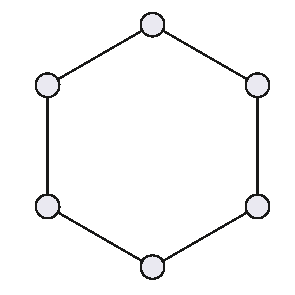
\includegraphics[width=0.3\linewidth]{/PSO/topology/pierscien.pdf} \label{fig: pso_topologies1}}
	\subfloat[]{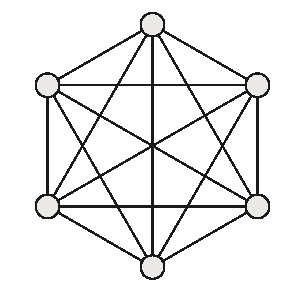
\includegraphics[width=0.3\linewidth]{/PSO/topology/global.pdf} \label{fig: pso_topologies2}}
	\subfloat[]{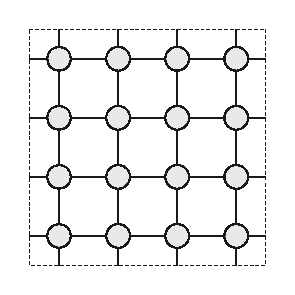
\includegraphics[width=0.3\linewidth]{/PSO/topology/neumann.pdf} \label{fig: pso_topologies3}}
	\captionsetup{justification=centering}
	\caption{}
	\label{fig: pso_topologies}
\end{figure}
Przyjęta topologia roju może mieć istotny wpływ na efektywność algorytmu. Topologie należące do rodziny gbest osiągają szybciej zbieżność, ale istnieje większe ryzyko na utknięcie w minimum lokalnym gdy funkcja celu nie jest unimodalna. Innymi słowy jest przynosi ona precyzyjniejsze rozwiązanie, ale mniej dokładnie przeszukuje obszar. Przy wykorzystaniu rodziny lbest efekt jest odwrotny. Ograniczona jest komunikacja jedynie do wąskiego grona sąsiadów przez co algorytm zbiega do rozwiązania wolniej, ale ma szansę przeszukać dokładniej wiekszy obszar.




\subsection{Zastosowania}
\subsection{Przykład teoretyczny}